\chapter{Existing solutions}
\label{cha:solutions}

In the previous chapter we discussed some of the philosophy surrounding distributive justice, and in this chapter we discuss some of the various ways those ideas have been made quantitatively precise.

In this chapter we consider some of the relevant formulations of the ways in which moral ideas about distribution have been mathemetised, primarily because our later developments extends from them and also ultimately contrasts against them.

We consider the following formulations:
\begin{itemize}
\item in section \ref{sec:solutions_VCG}, we consider the Vickrey-Clarke-Groves (VCG) mechanism,
\item in section \ref{sec:solutions_LMP}, we consider Locational Marginal Pricing (LMP),
\item in section \ref{sec:cooperative_game_theory_part}, we consider the Core and the Shapley Value,
\item in section \ref{sec:solutions_bargaining}, we consider Nash's bargaining solution concepts.
\DIFaddbegin \item \DIFadd{in section \ref{sec:envy_free_solutions}, we consider mathematical considerations associated with the concept of envy-freeness.
}\DIFaddend \end{itemize}

%These different approaches stem from different moral considerations, %and primarily reward participants with respect to different reference points that are briefly addressed in section \ref{sec:reference_points}.
%All of them tacitly respect formal equality (per section \ref{sec:formal_equality}), with bargaining and cooperative game theory concepts satisfying absolute efficiency requirements (per section \ref{sec:philosophy_efficiency}), and LMP often does so.

These different approaches stem from different moral considerations and have specific context and unique properties; we will introduce and discuss each of them in turn.
In the next chapter \ref{cha:new_solution} we attempt a new synthesis which brings many of these conceptual elements together.\\
Let us begin with the VCG mechanism.

\section{VCG}\label{sec:solutions_VCG}

In section \ref{sec:reference_points} we briefly presented the idea that people might be rewarded in proportion to their contribution to social welfare, above their absence, individually.
While this idea may be simple, its mathematisation has some surprising features.
The most direct mathemetisation of this idea is the Vickrey-Clarke-Groves (VCG) mechanism with Clark pivot.

The VCG mechanism (with Clark pivot) is an allocation process where each player is payed `transferable utility' (or money) equal to the impact that their presence has upon others (ie. their externality) in the decision process which selects an outcome that maximises the sum of utility.
Let us explain with some mathematics:

\subsection{The minimal VCG process - with Clark pivot}
If we frame the VCG process as a bidding process of $n$ agents over a possible set of outcomes $X$.
We assume that every agent $i$ has a valuation (or utility) $v_i$ for any outcome in $X$:
$$ v_i~:~X\rightarrow \mathbb{R}_{\ge 0} $$
The VCG bidding process asks every agent $i$ for their valuations and calculates the outcome that maximises the sum of the reported valuations:
$$ x^* = \argmax_{x\in X}\sum_{i=1}^{n}v_i(x) $$
This outcome is implemented and the process pays each agent $i$ the utility value $d_i$ (which may be positive or negative):
\begin{equation}\label{eq:VCG_payment_rule} d_i(v)=\sum_{j\ne i}v_j(x^*) - \max_{x'\in X}\sum_{j\ne i}v_j(x') \end{equation}
This value $d_i$ is the value that the player's presence adds to the utility of others minus the sum of the other player's utility which would have been obtained in the player's absence - ie. the player's externality.
In this equation the sum of other player's utility which would have been obtained in the player's absence $\max_{x'\in X}\sum_{j\ne i}v_j(x')$ is a special term called the 'Clark pivot', and in section \ref{subsubsection:groves_mechanisms} we discuss alternatives to this term.

\begin{example}
Consider a set of outcomes $X = \{A,B,C\}$ and three agents with valuations 
$$\begin{matrix}v_1(A) = 2\\v_1(B) = 4\\v_1(C) = 3\end{matrix}\quad\quad
\begin{matrix}v_2(A) = 4.5\\v_2(B) = 2\\v_2(C) = 1\end{matrix}\quad\quad
\begin{matrix}v_3(A) = 2\\v_3(B) = 1\\v_3(C) = 5\end{matrix}$$
In this context $x^* = C$ is implemented (as $\sum_{i=1}^nv_i(C)=9$ is the largest)\\And:
$\quad d_1 = 6-6.5 = -0.5 \quad\quad d_2 = 8-8 = 0\quad\quad d_3 = 4-6.5 = -2.5 $
\end{example}

\subsection{Discussion about VCG}
The VCG mechanism with Clark pivot might be seen as an straightforward way of assigning an outcome and allocating ethical payments; if a player's presence adds to the utility of others then they are positively compensated, and if a player's influence detracts from the utility of others then they are \DIFdelbegin \DIFdel{negatively compensated.
}%DIFDELCMD < 

%DIFDELCMD < %%%
\DIFdelend \DIFaddbegin \DIFadd{penalised in proportion.
}\DIFaddend Since the set of possible outcomes $X$ are arbitrary it is possible to consider the application of the VCG mechanism in a \DIFaddbegin \DIFadd{wide }\DIFaddend variety of contexts.
\DIFdelbegin \DIFdel{For instance, VCG has been considered as a mechanism for allocating physical and monetary outcomes in various contexts within electricity networks by various authors (such as \mbox{%DIFAUXCMD
\citep{FABRA200272, SESSA2017189, 8264596, 7512339}}\hspace{0pt}%DIFAUXCMD
), such as in auctions for bulk electricity generation, buying and selling energy storage products, and in procuring ancillary services.
}%DIFDELCMD < 

%DIFDELCMD < %%%
\DIFdelend However VCG has some particular advantages and disadvantages.
The first and most notable property is that VCG mechanisms have been demonstrated by \cite{roberts1979characterization, Lavi2008} to be \textit{truthful} or \textit{incentive compatible}, in \DIFaddbegin \DIFadd{the sense that }\DIFaddend that no single player can \DIFdelbegin \DIFdel{possibly }\DIFdelend \DIFaddbegin \DIFadd{positively }\DIFaddend gain by misreporting their valuations in the event that \DIFaddbegin \DIFadd{all other players are truthfully reporting their valuations, and in the event that }\DIFaddend the utility of the agents is \textit{quasilinear}.
An agent's utility is quasilinear if their utility is equal to their valuation of the outcome plus any transfers they receive, and hence their utility $u_i$ has form:
$$ u_i = d_i(v)+v_i $$
\DIFdelbegin \DIFdel{And thus if }\DIFdelend \DIFaddbegin \DIFadd{In this way if VCG's }\DIFaddend incentive compatibility induces the players not to bid strategically \DIFdelbegin \DIFdel{, then it reduces }\DIFdelend \DIFaddbegin \DIFadd{then it can reduce }\DIFaddend a potential overhead of their participation\DIFdelbegin \DIFdel{in the system, and also }\DIFdelend \DIFaddbegin \DIFadd{, and }\DIFaddend potentially eliminates a source of instability in the resulting system.

Another interesting property is called \textit{individual rationality}, in that no agent (assuming quasilinear utility) will ever be left with a net negative utility. Particularly if the utility of zero is regarded as the utility of non-participation, then individually rational means that everybody is left being better-off (or atleast not worse-off) by participating than they would be otherwise. Hence individual rationality is a possible articulation of ethical euvolentary negotiation (see chapter \ref{sec:reference_points}).

It is also worth noting that VCG mechanisms are also \textit{efficient} in the sense that the process actualises the utilitarian socially optimal solution $x^*(v) \in X$.

However, more negative features of VCG exist, one primary drawback of this mechanism is that it is not \textit{budget balanced}, in that it is possible that the amount of utility that is transferred between the players might not sum to zero.
Because of this an implementation of VCG might require regular budget injection to maintain and/or produce a budget surplus, hence sapping money from between the participants (see example).
As VCG may produce a budget surplus it is thus easy to note that the maximum amount of utility is not being given to the participants, and hence VCG is not efficient in the sense of maximising utility for the participants (see section \ref{sec:philosophy_efficiency}).
\DIFdelbegin \DIFdel{Although VCG is incentive compatiblefor individual strategisers }\DIFdelend \DIFaddbegin 

\DIFadd{Although VCG has a very positive property by being incentive compatible, }\DIFaddend it has some additional drawbacks \DIFdelbegin \DIFdel{, such as considered by \mbox{%DIFAUXCMD
\cite{ShohamLeytonBrown09}}\hspace{0pt}%DIFAUXCMD
:
as is potentially vulnerable to strategising coalitions, its implementation may involve imposing a lack of privacy for participants, and also }\DIFdelend \DIFaddbegin \DIFadd{and criticisms as noted by various authors \mbox{%DIFAUXCMD
\citep{ShohamLeytonBrown09,Rothkopf07}}\hspace{0pt}%DIFAUXCMD
, particularly:
}\begin{itemize}
\item	\DIFadd{The fact that VCG's truthfull equilibrium is a weak-equilibrium, and a player can misreport their valuations to harm others
}\item	\DIFadd{If generating or submitting a valuation in a VCG mechanism incurs some cost, over not participating, then it is no longer individually rational
}\item	\DIFadd{If the externalities and social optima $x^*$ are not solved exactly, but only approximately, then this will destroy the truthfulness property of VCG.
}\item	\DIFadd{If any players are budget-constrained (eg. they cannot afford to pay their true valuations for particular outcomes), then the truthfulness property is destroyed.
}\item	\DIFadd{If VCG mechanism does succeed in incentivising players to submit their true valuations, this is potentially has privacy and information disclosure issues.
}\item	\DIFadd{VCG is not completely immune from the possibility of cheating: by groups of players, by players submitting multiple bids under many names, or players who know that strategies in a series of VCG auctions may not be incentive compatible. etc.
}\item	\DIFadd{VCG may }\DIFaddend (depending on context) \DIFdelbegin \DIFdel{may }\DIFdelend also have higher computational complexity than other mechanisms.
\DIFdelbegin \DIFdel{These disadvantages of VCG have led it to be seldom implemented in practice, including in the context of electricity networks \mbox{%DIFAUXCMD
\citep{Rothkopf07, Ausubel2006}}\hspace{0pt}%DIFAUXCMD
}\DIFdelend \DIFaddbegin \end{itemize}

\DIFadd{Though some of these drawbacks and criticisms can be ameliorated, the VCG mechanism is widely discussed as potential mechanism in various real-world contexts, as we consider in section \ref{sec:vcg_real_world1}}\DIFaddend .

As VCG has positive and negative features, it is possible to ask if there are similar mechanisms which avoid some of the negative features.
But it is unfortunate, that some of these properties (incentive compatible, individually rational, budget balanced, and efficiency) are known to be impossible to combine in the general case (where there are a plurality of outcomes and the valuations are unrestricted), and these impossibility theorems are a feature in the study of \textit{Mechanism Design}.%(find a good source, of, myerson satterthwaite theorem)

\subsection{Mechanism Design, is there a better VCG?}

The VCG mechanism is a cornerstone \DIFdelbegin \DIFdel{component }\DIFdelend \DIFaddbegin \DIFadd{example }\DIFaddend in the field of Mechanism Design, and there exist many good sources giving extended discussions on the field - such as \cite{37377}.
But generally, Mechanism Design conducts the analysis of systems which select social outcomes based upon the result of strategic interactions of multiple parties with divergent interests.% and where each party has actual preferences over the possible outcomes, and also reported preferences over the outcomes.

One of the features of Mechanism Design that the VCG mechanism illustrates, is the potential for considering and apprehending the way in which a system is likely to behave between rational individually strategising agents.
This possibility extends beyond VCG, as it has been discovered that any system which is implemented between strategising agents can be altered such as to make it incentive compatible for them; this is called the revelation principle - see \cite{RePEc:ecm:emetrp:v:41:y:1973:i:4:p:587-601} \cite[Chapter~2.3]{37377}.
The revelation principle has various formulations, but generally, for any system there will some \DIFdelbegin \DIFdel{Nash-equilibria }\DIFdelend \DIFaddbegin \DIFadd{Nash equilibria }\DIFaddend in the interaction between the agents, and consequently an incentive compatible mechanism can be constructed by asking the agents for their true valuations and then implementing the corresponding \DIFdelbegin \DIFdel{Nash-equilibria }\DIFdelend \DIFaddbegin \DIFadd{Nash equilibria }\DIFaddend directly.
Unfortunately, it is sometimes the case that the \DIFdelbegin \DIFdel{Nash-equilibria }\DIFdelend \DIFaddbegin \DIFadd{Nash equilibria }\DIFaddend between strategising agents may not coincide with what is socially optimal for them; and the general difficulty of designing systems where the socially optimal outcome is always a \DIFdelbegin \DIFdel{Nash-equilibrium }\DIFdelend \DIFaddbegin \DIFadd{Nash equilibrium }\DIFaddend is rendered in some of the famous impossibility theorems in Mechanism Design. %And so, there are a series of strong impossibility proofs in mechanism design.

Some of the primary historic impossibility proofs in Mechanism Design concern voting and social choice systems, and notably include Arrow's impossibility theorem, and the Gibbard-Satterthwaite theorem.
But the difficulty does not necessarily recede even if monetary compensations between parties are included into consideration, such as per the Myerson-Satterthwaite theorem.
Another impossibility theorem was also proven by \cite{29088} to the effect of proving that there is no easy alternative to VCG - a mechanism which is incentive compatible, has unrestricted player preferences, has individual rationality, and implements a socially optimal outcome, in the case of quasilinear utilities.

In the evolving field of Mechanism Design there are several avenues of mitigating some of the impossibilities.

%\subsection{Navigating around impossibilities of Mechanism Design to a better VCG}

One of the main problems in applying VCG to electricity networks is the fact that it is not budget-balanced, and this raises a question of where the budget surplus/deficit should be channelled to/from.
Particularly if the money should be directed back to the participants in the electricity network, then it would destroy the incentive compatibility that was part of the scheme in the first place.
This is a direct consequence of the impossibility result of \cite{29088} and hence we are constrained to consider mechanisms which are suboptimal in relation to these qualities (budget balance, incentive compatibility, individually rational, and efficiency).
However it is also shown by \cite{YI201679} that there are no mechanisms which allow bounded deviations from the efficiency, incentive compatibility and budget-balance.

Thus a search for a better alternative than VCG needs to outright sacrifice or substitute some of these desirable properties.

Although we cannot go into too much detail about the field of Mechanism Design in this chapter (and the different kinds of impossibility theorems and kinds of incentive compatibility), we can highlight some interesting options.

\subsubsection{Redistribution in Groves mechanisms}\label{subsubsection:groves_mechanisms}

One potential avenue of averting the impossibility result is to discard the assumption that the player's valuation over outcomes are unrestricted, and recognise that some of the budget surplus/deficit can be redistributed without destroying the incentive compatibility property.

To frame this approach, we must make a technical distinction between a Groves mechanism and its particular instance - in the VCG mechanism.
A Groves mechanism is exactly the same as the VCG mechanism except instead of paying players per equation \ref{eq:VCG_payment_rule}, instead it pays them per:
\begin{equation}\label{eq:Groves_payment_equation} d_i(v)=\sum_{j\ne i}v_j(x^*) - C_{-i} \end{equation}
where $C_{-i}$ is some function that is independent of $i$'s reported preferences.
In this context it is notable that the VCG mechanism is a special case of a Groves mechanism \citep{10.2307/1914085} where $C_{-i}= \max_{x'\in X}\sum_{j\ne i}v_j(x')$.
Groves mechanisms are a class of mechanisms which include VCG, and are categorically incentive compatible. 

The challenge therefore is to derive optimal functions $C_{-i}$ which minimise the budget surplus/\DIFdelbegin \DIFdel{defecit }\DIFdelend \DIFaddbegin \DIFadd{deficit }\DIFaddend while maintaining individual rationality in the context of restricted player valuations.
For this purpose there has been significant discussion about deriving these $C_{-i}$ functions, also known as `VCG redistribution' rules.

One of the first to propose such a rule was \cite{Cavallo:2006:ODM:1160633.1160790}, who showed that much of the VCG surplus can be redistributed in a process of allocating a single physical object exclusively to one party (called `All-Or-Nothing' games), where it can be naturally assumed that any party has a utility of zero if they do not \DIFdelbegin \DIFdel{recieve }\DIFdelend \DIFaddbegin \DIFadd{receive }\DIFaddend the physical object.
This redistribution was possible primarily because there exists a simple constraint on player valuations - ie. not receiving the object has utility of zero.
\DIFdelbegin %DIFDELCMD < 

%DIFDELCMD < %%%
\DIFdelend Similarly in other situations where there are restrictions on the players\DIFaddbegin \DIFadd{' }\DIFaddend valuation over the outcomes, there is the potential for deriving \DIFaddbegin \DIFadd{different }\DIFaddend VCG redistribution rules.

However there are some difficulties with this approach, particularly it is known that even with VCG redistribution rules there will almost always be some remaining budget surplus, and even then the process of deriving optimal redistribution rules can be a difficult task --- even to the point where neural networks have been employed to approximate such functions (see \cite{DBLP:conf/atal/ManishaJG18}).

\subsubsection{Sacrificing efficiency with budget sinks}

Another avenue of averting the impossibility result is to sacrifice efficiency of outcome selection.
One of the simplest such schemes is given by \cite{Faltings2004b, Boi_faltings_patent}
who proceeds about the process of designing a \DIFdelbegin \DIFdel{non-pareto }\DIFdelend \DIFaddbegin \DIFadd{non-Pareto }\DIFaddend optimal VCG mechanism by splitting the population into two groups.
In this scheme, the VCG outcome from the first group is selected irrespective of the preferences in the second group and where the second group (the `sink') receives the budget surplus from the VCG mechanism applied to the first group.
This mechanism constitutes a budget balanced VCG-type mechanism which can be made more regular (suggested by \cite{10.1007/978-3-642-25510-6_14}) by randomly selecting an individual as the `sink', and splitting the budget surplus between the parties evenly without knowledge of who will be selected.

This kind of method of developing \DIFdelbegin \DIFdel{non-pareto }\DIFdelend \DIFaddbegin \DIFadd{non-Pareto }\DIFaddend optimal VCG mechanisms has been the subject of investigation by \cite{NATH2019673}, and the process is proven to necessarily need a `sink', although this such a sink can be randomly selected.
Notwithstanding it is expected that such a mechanism of randomly assigning a sacrificial `sink' could potentially be ethically dangerous; potentially falling afoul of Formal Equality ideas (see section \ref{sec:formal_equality}) as one member (or group of members) would be randomly singled out to equalise the budget surplus/\DIFdelbegin \DIFdel{defecit}\DIFdelend \DIFaddbegin \DIFadd{deficit}\DIFaddend .


%\subsubsection{switching to Baysean incentive compatability}

%is the source of the d'AVGA mechanism which allocates redistribution of the surplus bassed on baysean priors on player preferences.
%The addition of baysean priors also has links to bargaining, particularly with the work of Meyerson, and his bargaining games.
%Which in turn have been extened (by himself) to coalitional games, and also through some of his work to Harsanyi games. (CITE)
%Particularly through the introduction of baysean considerations other schemes can redily be made to be incentive compatable.
%However there are certain issues with supposing accurately known baysean priors (particularly if they are learnt from past behavior).

%And although incentive compatability is a noble objective in mechanism design, it is still subject to strategic manipulation, particularly in the context of the forming of coalitions.

%Coalition strategy proofness, has been proven to be quite generally a difficult concept to design, and in some cases has categorically proven to be impossible \cite{10.2307/2297048} without further elements, such as private information transfer and uncertainty.
%Although there has been some effort in designing and analysing the occurance of coalition proof mechanisms, these remain difficult.


\DIFaddbegin \subsection{\DIFadd{Applications of VCG to electricity systems}}\label{sec:vcg_real_world1}

\DIFadd{VCG has properties that make it attractive from from a theoretical standpoint, particularly its incentive compatability property brings the promise of alleviating the cost and potential system instability inherent between strategising agents that can be manifest in cases of market collapse.
Additionally it has a straightforward ethical interpretation, that is, as a policy of compensation for externality.
These advantages have led VCG to be often discussed, but its weaknesses have led to its being reportedly seldom implemented in practice, including in the context of electricity networks \mbox{%DIFAUXCMD
\citep{Ausubel2006,FABRA200272}}\hspace{0pt}%DIFAUXCMD
.
}

\DIFadd{In these discussions the primary difference between proposals of VCG application is the context of the events\&bids to which it is applied.
Thus VCG has been considered as a mechanism for allocating physical and monetary outcomes in various contexts within electricity networks by various authors:
}\begin{itemize}
\item	\DIFadd{VCG-like schemes have been considered as means of extracting truthfull preferences and allocating costings for demand across electric vehicle charging stations \mbox{%DIFAUXCMD
\citep{9263469}
}\hspace{0pt}%DIFAUXCMD
}\item	\DIFadd{VCG has been considered as a mechanism to determine compensation and induce truthfull information about consumer's inconvenience functions to demand response aggregators in demand response (DR) programs \mbox{%DIFAUXCMD
\citep{6965656}
}\hspace{0pt}%DIFAUXCMD
}\item	\DIFadd{VCG has been contrasted with other auction mechanisms in auctions for demand curtailment contracts under network uncertainty \mbox{%DIFAUXCMD
\citep{HEINRICH2021112335}
}\hspace{0pt}%DIFAUXCMD
}\item	\DIFadd{VCG has been considered as a possible auction mechanism for renewable energy aggregators to purchase and reward variable renewable energy generators for providing and truthfully reporting the distribution of their energy supply \mbox{%DIFAUXCMD
\citep{6120188}
}\hspace{0pt}%DIFAUXCMD
}\item	\DIFadd{VCG has been considered as a mechanism for allocating wholesale dispatch of electricity generation and consumption across a network:
	}\begin{itemize}
	\item	\DIFadd{such as between multiple network nodes with AC/DC links \mbox{%DIFAUXCMD
\citep{8939413,lmp2}}\hspace{0pt}%DIFAUXCMD
,
	}\item	\DIFadd{between multiple auctions for the supply of timely generation and ancillary services in a network \mbox{%DIFAUXCMD
\citep{7512339,Wang2022,SESSA2017189}
	}\hspace{0pt}%DIFAUXCMD
}\item	\DIFadd{as a means of allocating power and payments between generators and storage providers (such as EV owners) across stretches of time \mbox{%DIFAUXCMD
\citep{9483064,10.5555/2772879.2773528,7297853}
	}\hspace{0pt}%DIFAUXCMD
}\item	\DIFadd{and/or all these at once \mbox{%DIFAUXCMD
\citep{9203564}
	}\hspace{0pt}%DIFAUXCMD
}\end{itemize}
\end{itemize}

\DIFadd{In this way there are many possible context of VCG's application, however there are also some interesting innovations on VCG in the electricity context, such as:
VCG qualities can be improved is by considering mechanisms where VCG (or approximately VCG) payments are also in the Core (see Section \ref{sec:the_core_definition}) thus offering increased robustness properties against coalition strategising \mbox{%DIFAUXCMD
\citep{SESSA2017189,DBLP:journals/corr/abs-2012-05047,8264596}}\hspace{0pt}%DIFAUXCMD
.
Additionally there is specific VCG redistribution mechanisms discussed in the electricity context, particularly: such as using deep-learning to derive VCG redistribution rules in the context of EV bidding into a local energy market, as considered by \mbox{%DIFAUXCMD
\cite{9615367}}\hspace{0pt}%DIFAUXCMD
, or as a means of redistribution to minimise budget imbalance, such as described by \mbox{%DIFAUXCMD
\cite{8651383}}\hspace{0pt}%DIFAUXCMD
.
}




\DIFaddend \subsection{Summary and discussion of VCG}\label{subsec:summary_discussion_VCG}

The VCG mechanism frames a elegant ethical schema for distributive payments and is directly applicable to electricity systems.
Although it is incentive compatible, the primary practical draw-back to such a system is that it is not budget-balanced.
Unfortunately there is no easily implementable system that is like VCG \DIFdelbegin \DIFdel{that }\DIFdelend \DIFaddbegin \DIFadd{which }\DIFaddend is incentive compatible and \DIFdelbegin \DIFdel{is }\DIFdelend budget-balanced without forcing participants to potentially trade at a loss.

Notwithstanding it is a possible scheme for the trading of electricity and electric resources, and in the following chapter we will compare the allocations of power/money in randomly generated networks under VCG against other schemes.

One of the most \DIFaddbegin \DIFadd{central }\DIFaddend features about VCG, is that it is one of the most direct expressions of marginal payments - in that each participant is payed the marginal difference their presence causes to the well-being of the other participants \DIFaddbegin \DIFadd{in a utility maximising process}\DIFaddend .
This marginal \DIFdelbegin \DIFdel{quality }\DIFdelend \DIFaddbegin \DIFadd{difference consideration }\DIFaddend is shared by two other solutions of this chapter, particularly Locational Marginal Pricing (LMP) (section \ref{sec:solutions_LMP}) and Shapley Value (section \ref{subsec:the_shapley_value}).

One of the most notable qualities of VCG is that when it is scaled up to large numbers of participants (and no specific participants are particularly influential) then VCG often limits to another solution concept called \DIFdelbegin \DIFdel{Locatinal }\DIFdelend \DIFaddbegin \DIFadd{Locational }\DIFaddend Marginal Pricing, which often is budget balanced --- see \cite{NATH2019673, 8430852}.


\section{Locational marginal pricing}\label{sec:solutions_LMP}

In Section \ref{sec:reference_points} we briefly considered the notion that %moral and euvoluntary trading would result in normative market pricing; and potentially that 
the morality of a transaction could be framed with respect to the normal market prices.
There is potentially no greater framework for describing nominal market pricing in economic thought more influential than the concept of the \textit{margin} or more specifically \textit{marginal pricing}.

The idea that normal market trading should have any relation to moral trading was seen in John Locke's short essay Venditio where it is argued that a fair price for something is simply its normal market price at its location.\footnote{``... the market price at the place where he sells. Whosoever keeps to that in whatever he sells I think is free from cheat, extortion and oppression, ...'' \citep{locke2003locke}}
John Locke argues for this thesis, by considering that negotiating above market price for a good would be unethical primarily because any transaction would be taking advantage of ignorance or special circumstances of the buyer.
Conversely, negotiating below market price for a good would only incentivise reselling and allow others to profit at the original seller's loss\DIFdelbegin \DIFdel{.
Additionally}\DIFdelend \DIFaddbegin \DIFadd{, or alternatively}\DIFaddend , that selling below market price only to those who are needy is certainly a charity and hence cannot be required by justice\DIFdelbegin \DIFdel{, but that }\DIFdelend \DIFaddbegin \DIFadd{.
By these considerations, }\DIFaddend justice only requires offering no more than the same nominal market price for everybody.

While John Locke's arguments may or may not be convincing, it is useful to consider the transactions and pricing that would occur under idealised or normative euvoluntary trading as these prices might be considered moral in-themself (by Locke's argument), or provide a back-drop for the framing of more moral trading.
In section \ref{sec:solutions_bargaining} we consider mathematical schemas used to describe idealised normative bargaining between small numbers of participants, but in this section we describe some economic theory that has been used to describe normalised trading between large numbers of market participants.

%Unfortunately the determination of normalised trading, and normal market price is not nessisarily so easy to distill in practice.
Historic economic thought lends consideration to the idea that market prices can be described by combinations of factors, not limited to, supply and demand functions, market uncertainty, production costings and transport tariffs etc. and the combination of these may be related to the pricing and subsequent trading of the goods.
However, the way in which these factors have been seen to influence (or define) economic value has changed over time.

\subsection{A brief summary on the history of value}

In the history of economic thought, there was some general idea that the economic value of something (and hence its normal market price) should, in some way, be related to its usefulness in fulfilling human needs (however fickle or not) as things which are utterly useless seldom fetch any price.
%Even so far as to categorising into numbered classes different goods depending on their relation to satisficing needs (eg. \cite[Chapter 1]{mengerprinciples}).
%DIF < Such as where different needs (eg. hunger) require first-order goods (eg. bread) to satisfy them, and thoes require second-order goods to provide (eg. flour to make bread), and so on. 
%DIF > Such as where different needs (eg. hunger) require first-order goods (eg. bread) to satisfy them, and those require second-order goods to provide (eg. flour to make bread), and so on. 
But, above this, there was a difficulty explaining how it was that things which were most useful to satisfying needs often had little economic value, and things which were more useless were sometimes most economically valuable. This apparent contradiction is known as the water-diamond paradox, best put by Adam Smith:

%\begin{displayquote}
%The word VALUE, it is to be observed, has two different meanings, and sometimes expresses the utility of some particular object, and sometimes the power of purchasing other goods which the possession of that object conveys. The one may be called `value in use;' the other, `value in exchange.' The things which have the greatest value in use have frequently little or no value in exchange; and, on the contrary, those which have the greatest value in exchange have frequently little or no value in use. Nothing is more useful than water; but it will purchase scarce any thing; scarce any thing can be had in exchange for it. A diamond, on the contrary, has scarce any value in use; but a very great quantity of other goods may frequently be had in exchange for it.\cite{Smith1Gutenberg}
%\end{displayquote}

\begin{displayquote}
``The word VALUE, it is to be observed, has two different meanings, ... The things which have the greatest value in use have frequently little or no value in exchange; ... Nothing is more useful than water; but it will purchase scarce any thing; ... A diamond, on the contrary, has scarce any value in use; but a very great quantity of other goods may frequently be had in exchange for it.'' \citep{Smith1Gutenberg}
\end{displayquote}

In answer to this, there was promoted the idea that economic value reflects labor, as water is easy to procure but diamond is not so.
This `labor theory of value' was held by many authors (including Adam Smith\footnote{``The real price of every thing, what every thing really costs to the man who wants to acquire it, is the toil and trouble of acquiring it.''\cite{Smith1Gutenberg}}, David Riccardo\footnote{``The value of a commodity, or the quantity of any other commodity for which it will exchange, depends on the relative quantity of labour which is necessary for its production...''\cite[Section 1, Chapter 1]{Riccardo1Gutenberg}}, and many others) but most notably by Karl Marx:

\begin{displayquote}
``It suffices to say that if supply and demand equilibrate each other, the market prices of commodities will correspond with their natural prices, that is to say with their values, as determined by the respective quantities of labour required for their production'' \cite[Chapter 2]{marx1910value}
\end{displayquote}

And this idea, that the quantity of labour should (in some way) define market prices at market equilibrium, was subject to analysis and verification.
But ultimately the question of how to transform volumes of labour into competitive market prices became a difficult problem known as the `Transformation Problem'.

However, the various utilitarians of the 19th century viewed utility not only as a direction of moral efforts, but as a fundamental drive of human behaviour\footnote{for instance see Bentham: ``Nature has placed mankind under the governance of two sovereign masters, pain and pleasure.
It is for them alone to point out what we ought to do, as well as to determine what we shall do.''\cite{bentham1823introduction}}, including market behaviours such as price setting; and ultimately, this perspective yielded a new explanation for economic value.

The utilitarian perspective sought to explain market dynamics in terms of people's efforts to maximise their own utility (or more practically, profit), and in this context stable (and hence normal) market prices were associated with the equilibrium of those efforts.
This perspective yielded a link between market dynamics with the concept of the margin - or `marginalism'.

Although the concept of the margin was evidenced in some writings in the earlier half of the 19th century (such as in the works of Jules Dupuit and Hermann Heinrich Gossen), it took to the end of the century for the idea to become more thoroughly developed - see \cite{RePEc:ucp:jpolec:v:58:y:1950:p:307}.
Although there was much discussion about the relationship between the labour theory of value and marginalism at the end of the 19th century (such as reported by \cite{steedman2003socialism}) ultimately marginalism was adopted mainstream in the so-called 'marginal revolution', which has been identified (such as by \cite{marginalism1}) as defining the beginning of neoclassical economics.

The marginalist revolution saw that economic prices were not just equal to the summation of normal production costs\footnote{Such as promoted by Riccardo, ``The real and ultimate regulator of the relative value of any two commodities, is the cost of their production, and neither the respective quantities which may be produced, nor the competition amongst the purchasers.''\cite{Riccardo1Gutenberg}} (ultimately depending on the value of labor), but instead depended on the cost of production of the most marginal unit produced to meet demand.

\subsection{A sketch of marginalism}\label{subsec:marginal_price_sketch}

The idea of marginalism is best illustrated with a graph, in Figure \ref{fig_demand_supply} there is an illustration of a hypothetical market for a particular economic good, with many suppliers and many buyers.
In the figure we have the plotted the `Supply curve', identifying how many units of the good could be sustainably supplied to the market if the units sold for a particular price.
And we also have the `Demand curve', identifying how many units of the good would natrually be sold depending on the price which the goods sold at.
So for instance, at $\$30$ sale price per good, the market would be able to reliably support the production of $\sim 7$ goods, and the demand would be $\sim 23$, identifying a situation of unmet demand.

In this way, if the market is functioning ideally, then there is only one sensible outcome: that the goods should be sold in the number (and therefore at the price), that is at the intersection of the supply and demand curves - ie. the marginal price point.
For if there were more goods produced, then those excess units would be unsold hence their production would be unprofitable, and if there were less goods produced, then there would be unmet demand which would spur more production.
The graph shown might be indicative of a market for a finite resource (where increasing supply costs more), and where there is decreasing demand with increasing price.

Different sellers may choose different prices in a realistic market, however in this idealised situation where everybody is selling at the marginal price point, if any small individual seller tried to deviate from this price then it would be a disadvantageous for them.
For instance, If a seller tried to set a higher price than the marginal price then it would result in a failure to sell, or if a seller set a lower price then it would only result in less profit.
In this way, the marginal price point identifies an equilibrium of peoples utility (or profit) maximising efforts.

This kind of marginal analysis is a short sketch of the analysis and treatment in modern microeconomic texts (such as \cite{vohra_2020}).
This marginalist analysis is also widely regarded to resolve the water-diamond paradox, in that water is cheap because its marginal unit is cheap to produce.

Over time the marginalist synthesis was developed more comprehensively in the presence of many discussions and criticisms.
Particular criticisms attack the academic assertion that market participants are psychologically driven by rational utility maximisation (such as \cite{RePEc:ucp:jpolec:v:58:y:1950:p:307})\footnote{individual traders may be partially driven by irrationality such as fear, ignorance, gambling}, and the more pragmatic assertion that markets are approximately ideal and tend towards the stability of equilibrium (such as \cite{nla.cat-vn5739105})\footnote{as might be \DIFaddbegin \DIFadd{most directly }\DIFaddend witnessed in markets where is inherent uncertainty, notably in speculative markets such as stocks, housing and crypto-currency}.


\begin{figure}[]{}
    \centering
	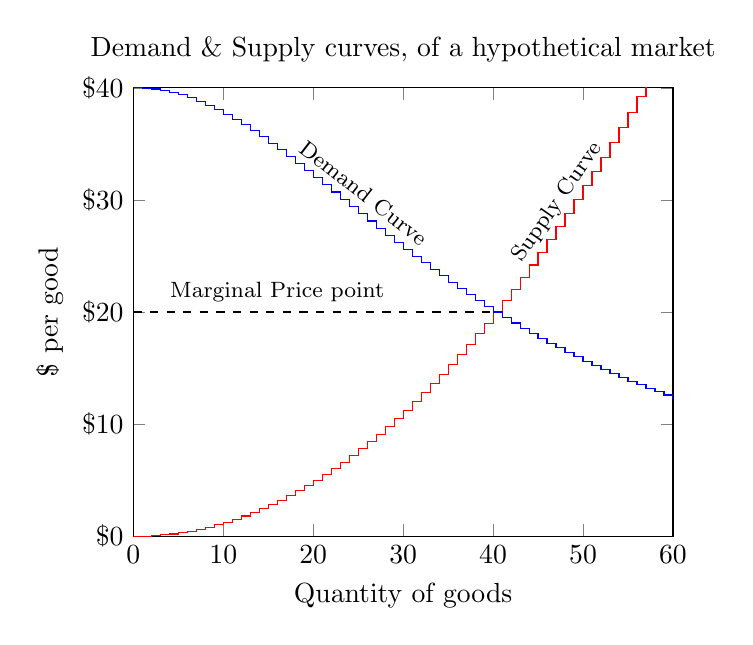
\begin{tikzpicture}
	\begin{axis}[
		title={Demand \& Supply curves, of a hypothetical market},
		xlabel={Quantity of goods},
		ylabel={\$ per good},
		xmin=0, xmax=60,
		ymin=0, ymax=40,
		%xtick={0,0.05,0.1,0.15,0.2,0.25},
		%ytick={30,35,40},
		yticklabel=$\$\pgfmathprintnumber{\tick}$,
		%ymajorgrids=true,
		grid style=dashed,
		xticklabel style={/pgf/number format/fixed},
	]
	\addplot[red] coordinates {
(0,0.0)(1,0.0)(1,0.012500000000000002)(2,0.012500000000000002)(2,0.05000000000000001)(3,0.05000000000000001)(3,0.11249999999999999)(4,0.11249999999999999)(4,0.20000000000000004)(5,0.20000000000000004)(5,0.3125)(6,0.3125)(6,0.44999999999999996)(7,0.44999999999999996)(7,0.6124999999999999)(8,0.6124999999999999)(8,0.8000000000000002)(9,0.8000000000000002)(9,1.0125000000000002)(10,1.0125000000000002)(10,1.25)(11,1.25)(11,1.5125000000000002)(12,1.5125000000000002)(12,1.7999999999999998)(13,1.7999999999999998)(13,2.1125000000000003)(14,2.1125000000000003)(14,2.4499999999999997)(15,2.4499999999999997)(15,2.8125)(16,2.8125)(16,3.2000000000000006)(17,3.2000000000000006)(17,3.6125)(18,3.6125)(18,4.050000000000001)(19,4.050000000000001)(19,4.5125)(20,4.5125)(20,5.0)(21,5.0)(21,5.5125)(22,5.5125)(22,6.050000000000001)(23,6.050000000000001)(23,6.612499999999999)(24,6.612499999999999)(24,7.199999999999999)(25,7.199999999999999)(25,7.8125)(26,7.8125)(26,8.450000000000001)(27,8.450000000000001)(27,9.1125)(28,9.1125)(28,9.799999999999999)(29,9.799999999999999)(29,10.5125)(30,10.5125)(30,11.25)(31,11.25)(31,12.012500000000001)(32,12.012500000000001)(32,12.800000000000002)(33,12.800000000000002)(33,13.612499999999999)(34,13.612499999999999)(34,14.45)(35,14.45)(35,15.3125)(36,15.3125)(36,16.200000000000003)(37,16.200000000000003)(37,17.1125)(38,17.1125)(38,18.05)(39,18.05)(39,19.0125)(40,19.0125)(40,20.0)(41,20.0)(41,21.0125)(42,21.0125)(42,22.05)(43,22.05)(43,23.112499999999997)(44,23.112499999999997)(44,24.200000000000003)(45,24.200000000000003)(45,25.3125)(46,25.3125)(46,26.449999999999996)(47,26.449999999999996)(47,27.612500000000004)(48,27.612500000000004)(48,28.799999999999997)(49,28.799999999999997)(49,30.012500000000006)(50,30.012500000000006)(50,31.25)(51,31.25)(51,32.512499999999996)(52,32.512499999999996)(52,33.800000000000004)(53,33.800000000000004)(53,35.1125)(54,35.1125)(54,36.45)(55,36.45)(55,37.8125)(56,37.8125)(56,39.199999999999996)(57,39.199999999999996)(57,40.612500000000004)(58,40.612500000000004)(58,42.05)(59,42.05)(59,43.5125)(60,43.5125)(60,45.0)(61,45.0)(61,46.51249999999999)(62,46.51249999999999)(62,48.050000000000004)(63,48.050000000000004)(63,49.6125)(64,49.6125)(64,51.20000000000001)(65,51.20000000000001)(65,52.8125)(66,52.8125)(66,54.449999999999996)(67,54.449999999999996)(67,56.1125)(68,56.1125)(68,57.8)(69,57.8)(69,59.51250000000001)(70,59.51250000000001)
		}node[pos=0.6](endofplotsquare){} ;
	\node [above, rotate=55] at (endofplotsquare) {\footnotesize Supply Curve};
	
	\addplot[blue] coordinates {
(0,40.0)(1,40.0)(1,39.97501561524047)(2,39.97501561524047)(2,39.900249376558605)(3,39.900249376558605)(3,39.77625854568055)(4,39.77625854568055)(4,39.603960396039604)(5,39.603960396039604)(5,39.38461538461539)(6,39.38461538461539)(6,39.119804400978)(7,39.119804400978)(7,38.8114008489994)(8,38.8114008489994)(8,38.46153846153846)(9,38.46153846153846)(9,38.0725758477097)(10,38.0725758477097)(10,37.64705882352941)(11,37.64705882352941)(11,37.187681580476465)(12,37.187681580476465)(12,36.69724770642202)(13,36.69724770642202)(13,36.178631995477666)(14,36.178631995477666)(14,35.634743875278396)(15,35.634743875278396)(15,35.06849315068493)(16,35.06849315068493)(16,34.48275862068965)(17,34.48275862068965)(17,33.88035997882477)(18,33.88035997882477)(18,33.26403326403326)(19,33.26403326403326)(19,32.63640999490056)(20,32.63640999490056)(20,32.0)(21,32.0)(21,31.35717785399314)(22,31.35717785399314)(22,30.71017274472169)(23,30.71017274472169)(23,30.061061531235325)(24,30.061061531235325)(24,29.411764705882355)(25,29.411764705882355)(25,28.764044943820224)(26,28.764044943820224)(26,28.1195079086116)(27,28.1195079086116)(27,27.479604980678403)(28,27.479604980678403)(28,26.845637583892618)(29,26.845637583892618)(29,26.218762802130275)(30,26.218762802130275)(30,25.6)(31,25.6)(31,24.990238188207734)(32,24.990238188207734)(32,24.39024390243902)(33,24.39024390243902)(33,23.800669393826702)(34,23.800669393826702)(34,23.222060957910017)(35,23.222060957910017)(35,22.654867256637168)(36,22.654867256637168)(36,22.099447513812155)(37,22.099447513812155)(37,21.55607948804311)(38,21.55607948804311)(38,21.02496714848883)(39,21.02496714848883)(39,20.50624799743672)(40,20.50624799743672)(40,20.0)(41,20.0)(41,19.506248095092957)(42,19.506248095092957)(42,19.024970273483948)(43,19.024970273483948)(43,18.556103218324154)(44,18.556103218324154)(44,18.099547511312217)(45,18.099547511312217)(45,17.655172413793103)(46,17.655172413793103)(46,17.22282023681378)(47,17.22282023681378)(47,16.802310317668677)(48,16.802310317668677)(48,16.39344262295082)(49,16.39344262295082)(49,15.996000999750061)(50,15.996000999750061)(50,15.609756097560975)(51,15.609756097560975)(51,15.234467983813378)(52,15.234467983813378)(52,14.86988847583643)(53,14.86988847583643)(53,14.51576321161261)(54,14.51576321161261)(54,14.171833480956598)(55,14.171833480956598)(55,13.837837837837839)(56,13.837837837837839)(56,13.513513513513514)(57,13.513513513513514)(57,13.198597648999794)(58,13.198597648999794)(58,12.892828364222401)(59,12.892828364222401)(59,12.595945679984254)(60,12.595945679984254)(60,12.307692307692308)(61,12.307692307692308)(61,12.027814320616427)(62,12.027814320616427)(62,11.756061719324025)(63,11.756061719324025)(63,11.49218890285509)(64,11.49218890285509)(64,11.235955056179774)(65,11.235955056179774)(65,10.987124463519313)(66,10.987124463519313)(66,10.745466756212224)(67,10.745466756212224)(67,10.510757102972573)(68,10.510757102972573)(68,10.282776349614396)(69,10.282776349614396)(69,10.06131111460462)(70,10.06131111460462)
		}node[pos=0.35](endofplotsquare){} ;
	\node [above, rotate=-38] at (endofplotsquare) {\footnotesize Demand Curve};


\addplot[dashed] coordinates {
(0,20.0)(40,20.0)
		}node[pos=0.4](endofplotsquare){} ;
	\node [above] at (endofplotsquare) {\footnotesize Marginal Price point};
	\end{axis}
	\end{tikzpicture}
	\vspace{-10pt}
	\caption{The Demand and Supply curves of a hypothetical market.}
	
	\label{fig_demand_supply}
\end{figure}


Notwithstanding, one of the most notable features of this neoclassical analysis is that the equilibrium marginal price point also maximises the sum of utility of those that participate in the market.
This can be seen from Figure \ref{fig_demand_supply} where all the buyers who value the goods the most are provided from all the sellers who can supply those goods at lowest cost up until the marginal point where no further trade is viable.

This point of utility maximisation is seen in Neoclassical analysis more generally, where market equilibrium prices (at and/or between markets) occur at the point of the maximisation of the sum of utility. Indeed, the process of mathematically deriving these marginal prices developed into a kind of calculus, where the marginal prices fall out as Lagrange multipliers in the process of maximising the sum of utility.

To see this, consider the curves in figure \ref{fig_demand_supply} where the Demand function is\\ $D(x) = \frac{40}{1+(x/40)^2}$ and the Supply function is $S(x) = 20(x/40)^2$.

From these functions\footnote{We could, more directly, observe that by solving $S(x)=D(x)$ we get $x=40$.} we construct the utility of the buyers and sellers as:
$$U_d(x) = \int_0^x\frac{40}{1+(z/40)^2}dz \quad\quad\text{and}\quad\quad U_s(x) = -\int_0^x20\left(\frac{z}{40}\right)^2dz$$
In this context $U_d(x)$ represents the sum of utilities of the buyers for $x$ goods sold to them\footnote{The equation is an integration because, if $x$ is zero, then the utility of the buyers is zero because there are no goods transacted, if $x$ is 1 we might imagine that the good goes to the buyer who values it the most and whose utility is given the maximum leftmost point on the demand curve, if $x$ is 2 then the utility of the buyers is the sum utility of the one who values it the most and the second most, if $x$ is 3 then it is the sum of utilities of the 3 most buyers, etc.} and $U_s(x)$ represents the sum of costs suffered by the sellers for $x$ goods produced by them\footnote{The equation is an integration because, if $x$ is zero, then there are no goods produced and no costs to the sellers, if $x$ is 1 then we might imagine that the good was produced by the cheapest seller, who's cost is given by the leftmost point on the supply curve, if $x$ is 2 then the utiltiy is the sum of costs of the two chepest sellers, etc.}.

If the amount of the goods bought is $a$ and the amount supplied is $b$ then we can construct the utility function as $U(a,b) = U_d(a) + U_s(b)$
and to maximise this subject to the conservation constraint $a=b$, we use lagrange's method of multipliers, and form lagrangian:
$L(a,b,\lambda) = U_d(a) + U_s(b) + \lambda(b-a)$
$$\frac{\partial L}{\partial a} = \frac{40}{1+(a/40)^2} - \lambda = 0 \quad\quad\text{thus:}\quad\quad a = 40\sqrt{40/\lambda - 1}$$
$$\frac{\partial L}{\partial b} = -20\left(\frac{b}{40}\right)^2 + \lambda = 0 \quad\quad\text{thus:}\quad\quad b = 40\sqrt{\lambda/20}$$
substituting into the constraint $a=b$ gives $\lambda=20$ and thus $a=b=40$\\
In this way the Lagrange multiplier on the conservation constraint gives the marginal price of the good - which is also called the `shadow price'.

The general development of the mathematics is slightly beyond our scope here, but the general process is:
\begin{enumerate}
\item Formulate the utility function from all the market participants, including all variables
\item Form an optimisation problem for utility maximisation with appropriate conservation constraints
\item Solve the optimisation problem, and record the Lagrange multipliers of the conservation constraints as shadow prices.
\end{enumerate}
This process, of using calculus to determine nominal prices has been proposed in the electricity space \DIFdelbegin \DIFdel{in recent years }\DIFdelend - such as by \cite{lmp1, lmp2, lmp4, game3}.
Particularly as the process of maximising utility on an electricity grid is a well known problem called the `Optimal Power Flow' problem (OPF), where the power conservation constraint at each bus of the network, identifies the marginal price of electrical power on that bus.
This particular scheme is called `Locational Marginal Pricing' (LMP); and we will investigate and compare against it against other solutions in section \ref{sec:features}.

Particularly, we note that LMP has been implemented for real-time-pricing of transmission power in some existing electricity systems - such as reported by \cite{WANG2015695,zonal}.
And that although LMP is like VCG in that it is ultimately not budget balanced, unlike VCG there are specifically identifiable cases where budget imbalance occurs, particularly in the context of network \textit{congestion} - see \cite{lmp2}.




\subsection{\DIFdelbegin \DIFdel{Summary and discussion }\DIFdelend \DIFaddbegin \DIFadd{Applications }\DIFaddend of \DIFdelbegin \DIFdel{locational marginal pricing}\DIFdelend \DIFaddbegin \DIFadd{Locational Marginal Pricing to electricity systems}\DIFaddend }

\DIFaddbegin \DIFadd{In the historical context of power systems, one of contested and contrasted options in electricity market structure was Discriminatory/Pay-As-Bid-Pricing and Uniform/Marginal Pricing.\mbox{%DIFAUXCMD
\citep{wolfram1999electricity,comparrison1,HAGHIGHAT2012350,griffin2009electricity,su13063429,FABRA200272}
}\hspace{0pt}%DIFAUXCMD
In the electricity market context, generator companies `bid' into a system an offer consisting of what amount of power/s they can supply and at what amount they expect to be paid for the respective dispatch.
This can occur in a day-ahead market structure, where a central and Independent System Operator (ISO) collects bids and accepts them to meet anticipated demand the following day.
The primary question between Pay-As-Bid and Marginal Pricing is if the generator companies who's bids are accepted should simply be paid their monetary bid amount, or should directly be paid the cost of the marginal unit of power dispatched.
}

\DIFadd{While it may initially seem as if Pay-As-Bid pricing would be most reasonable, it is demonstrated that strategic equilibrium in the bidding of generator companies should ideally yield the respective Marginal Pricing values anyway (as already indicated in section \ref{subsec:marginal_price_sketch} and demonstrated in \mbox{%DIFAUXCMD
\cite{klemperer1999auction}}\hspace{0pt}%DIFAUXCMD
).
In this way, the question between Pay-As-Bid and Marginal Pricing is if the market operator should shortcut the strategising of generator companies, and thus afford the marginal prices directly.
}

\DIFadd{This discussion between Pay-As-Bid-Pricing and Marginal Pricing was mostly discussed throughout the deregulation process of electricity networks that occurred in many countries throughout the 80's to the 2000's \mbox{%DIFAUXCMD
\citep{deregulation}}\hspace{0pt}%DIFAUXCMD
, and was also reconsidered in the aftermath of the California electricity crisis. \mbox{%DIFAUXCMD
\citep{california1,KAHN200170}
}\hspace{0pt}%DIFAUXCMD
However, in real terms, Marginal Pricing of some sort is more the commonly implemented rule, as opposed to Pay-As-Bid, and a centralised Marginal Pricing rule is a direct precursor to a locationally variant Marginal Pricing rule - that is, Locational Marginal Pricing (LMP).
}

\DIFadd{However with the implementation of LMP, there are additional factors that may need to be addressed in practical settings, such as:
}\begin{itemize}
\item	 \DIFadd{LMP schemes can be considered to various levels of refinement, such as between zonal and nodal levels \mbox{%DIFAUXCMD
\citep{WANG2015695,zonal} }\hspace{0pt}%DIFAUXCMD
where the degree of refinement and the boarders between zones potentially have practical and social consequences, and influence computational difficulty in the calculation.
}\item	\DIFadd{LMP is inherently built upon an electrical network optimisation scheme which potentially includes various elements of complexity. For instance, LMP prices can be built upon a DC approximation model of electricity flow (it computationally the more simple), but in principle various AC models (and their relaxations) are possible candidates. \mbox{%DIFAUXCMD
\citep{Wang1}
}\hspace{0pt}%DIFAUXCMD
}\item	\DIFadd{LMP method does not directly incorporate or account for discontinuous variables. This factor is most notable in the Unit Commitment (UC) stage of generators scheduling to meet demand, as generator state cannot always be continuous (such as on/off state). For these discontinuous parameters, LMP prices can be supplemented by side payment methods to support the dispatch of power. There exists discussions about different  schemes to calculate and organise these side-payments. \mbox{%DIFAUXCMD
\citep{8871218,johnson1997equity}
}\hspace{0pt}%DIFAUXCMD
}\item	\DIFadd{Locational Marginal Prices vary over time and between zones/nodes of the network which are subject to congestion and whereby congestion rents are extracted. These congestion rents need to be redistributed and secondary markets may be implemented for these as a consequence, notably Financial Transmission Rights (FTR) auction processes. 
Financial Transmission Rights are financial instruments which ISOs offers to generator companies to hedge against LMP volatility \mbox{%DIFAUXCMD
\citep{ftr_article1}}\hspace{0pt}%DIFAUXCMD
, these FTRs then alter the pricing landscape in electricity network context which then has potential secondary effects. \mbox{%DIFAUXCMD
\citep{WU2022121893}
}\hspace{0pt}%DIFAUXCMD
}\item	\DIFadd{LMP is static for a single timeframe and is not completely incentive compatible, and these factors yield real world strategising in electricity markets \mbox{%DIFAUXCMD
\citep{hu2005empirical,dungey2018strategic}}\hspace{0pt}%DIFAUXCMD
, and this is most notably true around the mechanism of revising bids or `rebidding', over a finite time horizon \mbox{%DIFAUXCMD
\citep{8054716}}\hspace{0pt}%DIFAUXCMD
.
}\item	\DIFadd{LMP is tacitly based on full and static information, and although there is some attempt to integrate uncertainty into the marginal price mechanism itself \mbox{%DIFAUXCMD
\cite{9299487,8910409}}\hspace{0pt}%DIFAUXCMD
, there is a broader discussion about different ways to accommodate uncertainty from historical data into the design and operation of electricity systems generally \mbox{%DIFAUXCMD
\citep{en15030825}}\hspace{0pt}%DIFAUXCMD
. In-practice the value of short-term demand/supply uncertainty and imbalance is not reflected in Locational Marginal Prices, but can be addressed via secondary ancillary support markets - such as providing frequency stability.\mbox{%DIFAUXCMD
\citep{ELA201651}
}\hspace{0pt}%DIFAUXCMD
}\end{itemize}

\DIFadd{These considerations extend primarily from there being factors (discontinuous, diachronic, probabilistic, etc.) that are outside of the Marginal Pricing calculus that cannot (or are not often, or easily) incorporated, thus adding to the complexity of LMP in real-world markets.
Notwithstanding these considerations, LMP has particular advantages such as its ability to be computed and its linkage to economically relevant rationale, that means that it is actually implemented over other schemes in practice \mbox{%DIFAUXCMD
\citep{zonal}}\hspace{0pt}%DIFAUXCMD
, and serves us as a benchmark to compare other schemes against. 
}


\subsection{\DIFadd{Summary and discussion of Locational Marginal Pricing}}

\DIFaddend Locational Marginal Pricing is a historic example of an economic framework of integrating market conditions (supply and demand information) to give equilibrium price points.
It can be seen to provide a description of normal trading value, and thence (perhaps) moral trading value.

Locational Marginal Pricing and VCG provide some of the most direct expressions of Marginalism as a concept, and (as considered in section \ref{subsec:summary_discussion_VCG}) one can limit to the other for large markets.
Particularly VCG rewards participants with economic incentives equal to their direct impact on group wellbeing above their absence, whereas Locational Marginal Pricing can be seen as providing participants with economic incentives in proportion to their presence's marginal (or incremental) impact on group wellbeing.

With VCG it is directly considered what the notion of absence means, particularly the direct difference the presence of a participant makes is in relation to the affect the participant's utility brings upon the social utility maximum.
However the notion of absence under LMP may be less clear; the marginal prices are the rate of incremental utility value of additional goods at the respective location, which in turn is the incremental rate that each participant's presence brings at that location.

In the following chapter \ref{cha:new_solution}, LMP and VCG are implemented and the differences between the two can be witnessed.
%Both are expressions of marginalism, in that both revolve around the socially optimal utility point, and reward participants with respect to their contribution to it.

Both LMP and VCG root their concept of value in the idea of marginal contribution implicitly with respect to some notion of absence. However, in other contexts it may not be clear what this means, in section \ref{sec:solutions_bargaining} we outlay some solutions concepts which which embrace this ambiguity.

However before we move to section \ref{sec:solutions_bargaining}, we notice that both LMP and VCG only treat every player individually, but neglect any consideration of possible groups of players and their influence.
And so, in the next section \ref{sec:cooperative_game_theory_part} we consider solution concepts which explicitly consider groups and their marginal contributions.



\section{Cooperative game theory}\label{sec:cooperative_game_theory_part}

In section \ref{sec:reference_points} we considered the idea that groups of people could be afforded what they could achieve `by themself'.
And this idea is most directly articulated by the \textit{Core} of cooperative game theory.
In that same section we also mentioned the idea that people could be rewarded for their contribution under uncertainty about the presence of other group members, and that this idea was most directly articulated by the \textit{Shapley Value} of cooperative game theory.

Both of these ideas directly or implicitly consider possible groups and how much value each group has `by itself', and this is directly the ground of cooperative game theory.

The basic elements of a classic cooperative game are that there is a set of players or individuals $N=\{1,2,\dots n\}$ and a function $v: S\subseteq N \rightarrow \mathbb{R}$ with $v(\emptyset)=0$ called the \textit{characteristic function}.
The characteristic function identifies in some sense the `worth' or `value' of any group of players (a `coalition') which might be interpreted in terms of utility or monetary value.
In this context, one aim of cooperative game theory is to develop schemes (or `solution concepts') which split the wealth achieved if everybody cooperated (that is $v(N)$) between all the players.

Fundamentally, this kind of analysis hinges on there being a clearly defined concept and determination of the value of each possible group (ie. the characteristic function), however it is not always the case that there is such a clearly defined notion.
Consider the words of Lloyd Shapley about the characteristic function:

\begin{displayquote}
``The idea is to capture in a single numerical index the potential \underline{worth} of each coalition of players...

With the characteristic function in hand, all questions of tactics, information, physical transactions, etc., are left behind. The characteristic function is primarily a device for dividing the difficulties -- for eliminating as many distractions as possible in preparation for the confrontation with the indeterminacy of what we have called the ``n-person problem''. Engrossed with this problem, many authors writing after von Neumann and Morgenstern have begun by basing their solution concepts on the characteristic function above, with no initial concern for the concrete rules of the game, in strategic or extensive form.

Unfortunately, not all games admit a clean separation between strategic and coalitional questions, and for those that do not the characteristic function approach must be modified or abandoned.''\\
\citep{ShapleySchubikCharacteristicFunction}
\end{displayquote}

In this light, there exist situations where the `worth' of a coalition may be ambiguous such as where there are strategic considerations between possible coalitions, and there is no uniquely defined value that members of a coalition could/would achieve.
However, some situations do cleanly admit a definable `worth' for groups of individuals, for instance, the Characteristic function may identify the amount of money that members of a coalition could, and unambiguously would, achieve by working for themself irrespective of the actions of those not belonging to the coalition.

In these cases, if everybody works together to achieve some maximal sum of money there are a set of possible ways the money can be divided between everybody.
One of the most natural divisions is that every subgroup should be given at least more than they could feasibly achieve by working for by themself as a group.
And this is an allocation most naturally described by the \textit{Core}.

\subsection{The Core}\DIFaddbegin \label{sec:the_core_definition}
\DIFaddend 

The Core is an example solution concept for cooperative games, in that for any set of players $N=\{1,2,\dots n\}$ and any characteristic function $v: S\subseteq N \rightarrow \mathbb{R}$ with $v(\emptyset)=0$, the Core is a set of possible payoff allocations to each of the players $C(v)$ in which each subgroup is given at least the value of the characteristic function for that subgroup:

$$ C(v) = \left\{x\in\mathbb{R}^n : \sum_{i\in N}x_i=v(N); \sum_{i\in S}x_i \ge v(S), \forall S\subseteq N \right\}$$

The Core is the set of possible allocations such that for any group of individuals, the sum allocated to the group is greater than what the group could achieve by working by themself.
The allocations in the Core might be seen to have a kind of stability property - in that no coalition would have an incentive to leave the grand coalition. One major drawback about the Core is that it does not determine a unique outcome, but potentially a range of outcomes or potentially none at all, depending on the cooperative game.

Indeed the Core may be empty, and in this case no solution can have the same kind of desirable stability, however there are alternative allocations that minimise this shortcoming.
Most notably, the \textit{least-Core} solution concept.

The least-Core solution concept is a particular instance of the \textit{strong $\epsilon$ Core} which is very similar to the Core, and is defined as follows:
$$ C_\epsilon(v) = \left\{x\in\mathbb{R}^n : \sum_{i\in N}x_i=v(N); \sum_{i\in S}x_i \ge v(S)-\epsilon, \forall S\in N \right\}$$
The strong $\epsilon$ core is the set of allocations in which each coalition is allocated atleast their value minus some constant $\epsilon$.
The strong $\epsilon$ Core can be defined for positive and negative $\epsilon$ values, it will certainly be non-empty for very large and positive $\epsilon$ values and certainly be empty for very negative $\epsilon$ values.
In this way we can consider the limiting case between these two, the smallest value of $\epsilon$ in which the strong $\epsilon$ Core is non-empty --- and this is the least-core, see \cite{doi:10.1287/moor.4.4.303}.
The least-core is therefore always non-empty and may even identify a singular solution point, which that can be said to identify the point of minimum `dissatisfaction' between the groups.

The Core is an intuitive solution concept in the context where the characteristic function identifies the `worth' of individuals and groups `by-themself' and the dynamics are driven by this isolation mechanic.
However in other cases the `worth' identified by the characteristic function may be in the context of cooperation with the others.
And in this context the Core is not the only solution concept worth considering.

\subsection{The Shapley Value}\label{subsec:the_shapley_value}

The \textit{Shapley Value} is another specific and well known solution concept in cooperative game theory.
Particularly the Shapley Value allocates to each individual the average contribution they would add across the possible coalitions to which they could join.

Particularly, for any coalition $S$ which does not include a player $i$, then player $i$'s marginal contribution is $v(S\cup\{i\}) - v(S)$. If we average such contributions for coalitions of size $k$:
\begin{equation}\label{eq:shapley_value2}
\hat{v}_{i,k} = \frac{1}{\binom{n-1}{k}}\sum_{S\subseteq N\setminus \{ i\} , |S|=k} %\frac{(n-|S|-1)!\,|S|!}{(n-1)!}
(v(S\cup\{i\})-v(S))
\end{equation}
Then we have the average marginal contribution of player $i$ to coalitions of size $k$, and if we average this over coalitions of different size, we get the Shapley Value:
\begin{equation}\label{shap2} \varphi_i(\langle N,v\rangle) = \frac{1}{n}\sum_{k=0}^{n-1}\hat{v}_{i,k} \end{equation}
Or more directly as:
\begin{equation}\label{shap1_X}\varphi_i(\langle N,v\rangle) = \sum_{S\subset N, i\notin S}\frac{(n-|S|-1)!\,|S|!}{n!}(v(S\cup\{i\})-v(S))\end{equation}
The Shapley Value is an averaging over a players marginal contributions, which is thus a unique allocation for any cooperative game.

The Shapley Value for a player can also be formulated as being the expected marginal contribution across all join ordering processes.
So for instance, if we let $\pi(N)$ denote the set of all ordered permutations of the player set $N$ and if we denote $Pre^i(O)$ as the set of predecessors of player $i$'s addition in that ordering $O\in \pi(N)$. Then the Shapley Value can be expressed as the average marginal contribution across orderings, see \cite{weber_1988}:
\begin{equation}\label{shapley_value3}
    \varphi_i(\langle N,v\rangle) = \frac{1}{n!}\sum_{O\in\pi(N)}v(Pre^i(O)\cup\{i\})-v(Pre^i(O))
\end{equation}

In this way the Shapley Value for a player can be directly expressed as the average marginal contribution across possible join order processes.
%Or alternatively,
%\begin{equation}\label{eq:shapley_value}
%    \varphi_i(\langle N,v\rangle)= \frac{1}{n}\sum_{S\subseteq N\setminus\{i\}} \binom{n-1}{|S|}^{-1} \left(v'(S\cup\{i\})-v'(S)\right) 
%\end{equation}

The Shapley Value has perhaps some moral intuition behind it - rewarding each person in proportion to what they would add across any ordering that the coalition could form.
But more than that, the Shapley Value has been derived from different sets of quite intuitive axioms.
For instance:

\begin{itemize}
\item	\textbf{Efficiency}: That the total dividend is broken up, $\sum_i\varphi(\langle N,v\rangle)_i = v(N)$
\item	\textbf{Symmetry}: If two players $i$ and $j$ are substitutes and contribute the same to all coalitions, such that if $v(S\cup i)=v(S\cup j)~~\forall S\subseteq N\setminus\{i,j\}$, then $\varphi(\langle N,v\rangle)_i = \varphi(\langle N,v\rangle)_j$
\item	\textbf{Dummy Player}: A player $i$ is a dummy player if the amount that $i$ contributes to any coalition is the amount that $i$ is able to achieve alone (i.e.\ $v(S\cup \{i\})-v(S)=v(\{i\})~~\forall S\subseteq N\setminus\{i\}$) then $\varphi(\langle N,v\rangle)_i=v(\{i\})$
\item	\textbf{Additivity}: That for any two games, the imputation for the two together is the sum of the imputations in each, for any $v_1$ and $v_2$, $\varphi(\langle N,v_1+v_2\rangle)=\varphi(\langle N,v_1 \rangle) + \varphi(\langle N,v_2\rangle)$
\end{itemize}

These axioms might seem pretty reasonable and they lead uniquely to the Shapley Value allocation - per \cite{Shapley1953a}; additionally there are other possible sets of axioms which also lead to the Shapley Value aswell.
These axioms (particularly Efficiency and Symmetry axioms) relate directly to morally relevant points raised in the philosophy chapter \ref{sec:philosophy} (Efficiency and formal equality conditions respectively).

In considering the Shapley Value, there is the additional question of when the Shapley Value is in the Core - and thus has that particular stability that would disincentivise any subgroup from leaving.
One example case where the Shapley Value is always in the Core is the case of Convex cooperative games, see \cite[Chapter 6]{RePEc:cup:cbooks:9781107691322}:
A cooperative game is \textit{convex} if the value that two coalitions together has is greater than the value of their parts minus the value of their intersection, ie. iff:
\begin{equation}
    \forall S,T\subset N \quad v(S\cup T) \ge v(S)+v(T)-v(S\cap T)
\end{equation}
Which is potentially a common condition in which each coalition is informally `greater than the sum of its parts'.
We consider an example:

\begin{example}
Consider player set $N=\{1,2,3\}$ with characteristic function:\\
$v(S)=\left(\prod_{i\in S}i\right)-1$ (ie. the multiplication of their player numbers minus one).\footnote{We are assuming that the product over an empty set is one.}\\
Solve for the Shapley Value, and show that it is efficient and also in the core.
\end{example}

\begin{solution}
To calculate the Shapley Value for player $C$, we consider the marginal contributions it can make to other coalitions:\\
$ v(\{C\})-v(\emptyset) = 2-0 = 2, \quad\quad\quad v(\{C,A\})-v(\{A\}) = 2-0 = 2$\\
$ v(\{C,B\})-v(\{B\}) = 5-1 = 4, \quad v(\{C,A,B\})-v(\{A,B\}) = 5-1 = 4  $\\
Thus the Shapley Value for player $C$ is:
$\varphi_C = \frac{1}{3}\left(2 + \frac{1}{2}(2+4) + 4\right) = 3$, and contiuing for the other players gives:
$\varphi_A = 0,\quad\varphi_B = 2$\\
The Shapley Value is efficient as: $\varphi_A+\varphi_B+\varphi_C = 5 = v(\{A,B,C\})$\\
and also in the Core, as it is true that:\\
$\varphi_A+\varphi_B=2\ge v(\{A,B\})=1$\\
$\varphi_A+\varphi_C=3\ge v(\{A,C\})=2$\\
$\varphi_B+\varphi_C=5\ge v(\{B,C\})=5$\\
It is also simple enough to verify that the cooperative game is convex.

\end{solution}

\subsection{Summary and applications to electricity systems}

Cooperative game theory concepts centre on the consideration of groups and how reward or surplus utility should be divided among members, and particularly the Shapley Value is most famous.

Indeed the Shapley Value has been considered as a potential mechanism for pricing in the various facets of electricity system operation. Such as: 
\DIFaddbegin \begin{itemize}
\item	\DIFadd{Credits in }\DIFaddend demand response participation \citep{DBLP:journals/tsg/OBrienGR15,electronics8010048,WANG201972}
\DIFdelbegin \DIFdel{, compensation }\DIFdelend \DIFaddbegin \item	\DIFadd{Compensation }\DIFaddend for the aggregation of power \citep{Perez-Diaz:2018:CEV:3237383.3237484,6520960}
\DIFdelbegin \DIFdel{, allocating }\DIFdelend \DIFaddbegin \item	\DIFadd{Allocating }\DIFaddend transmission costs and losses \citep{ip-gtd_20020005,SHARMA201733}
\DIFdelbegin \DIFdel{, allocating }\DIFdelend \DIFaddbegin \item	\DIFadd{Dividing }\DIFaddend profits for retailers and \citep{ACUNA2018161,WANG201972}
\DIFdelbegin \DIFdel{, allocating }\DIFdelend \DIFaddbegin \item	\DIFadd{Allocating }\DIFaddend surplus and savings in microgrids \DIFdelbegin \DIFdel{\mbox{%DIFAUXCMD
\citep{WU2017384} }\hspace{0pt}%DIFAUXCMD
and allocating }\DIFdelend \DIFaddbegin \DIFadd{\mbox{%DIFAUXCMD
\citep{WU2017384,LOPRETE2016524}
}\hspace{0pt}%DIFAUXCMD
}\item	\DIFadd{Sharing }\DIFaddend costs in distribution and embedded networks \citep{archie_paper1,8226810,10.1007/978-3-642-40776-5_19,6840296,DBLP:journals/corr/abs-1903-10965,AzuatalamCV_PowerTech2019}
\DIFdelbegin \DIFdel{.
}\DIFdelend \DIFaddbegin \end{itemize}
\DIFaddend 

In each of these cases, the primary difference is the context of application and the specific way in which the characteristic function is constructed.

\DIFdelbegin \DIFdel{Just like in LMP and VCG, the Shapley Value is also evidently a marginal approach , }\DIFdelend \DIFaddbegin \DIFadd{The Shapley Value has notable strengths and weaknesses, particularly the simplicity of its axioms have obvious appeal, and similar to LMP and VCG it is a more expansive marginalist approach (}\DIFaddend as it is expressible the an average \DIFdelbegin \DIFdel{marginal contribution across possible groups (}\DIFdelend \DIFaddbegin \DIFadd{over a larger range of marginal contributions }\DIFaddend by equations \ref{shap2} or \ref{shapley_value3})\DIFaddbegin \DIFadd{.
However a primary drawback of the Shapley Value in practice is the difficulty of computing it as calculating all of the marginal contributions of all players to the $2^n-1$ possible coalitions is identified as being rapidly difficult to scale to sizes of participants on realistic networks.
This drawback has attracted attention and attempts at remediation, such as employing techniques of sample-bassed approximations (see citations in Section \ref{sec:shapley}) or approaches that employ techniques like player clustering \mbox{%DIFAUXCMD
\cite{DBLP:journals/corr/abs-1903-10965}}\hspace{0pt}%DIFAUXCMD
.
}\DIFaddend 

%Informally the difference between VCG, LMP and the Shapley Value can be seen as a difference between the allocation of reward: equal to contribution to the grand coalition, in-proportional to marginal contribution to the grand coalition, or equal to contribution not just to the grand coalition.

\DIFdelbegin \DIFdel{There there is much more which could be said about cooperative game theory, but }\DIFdelend \DIFaddbegin \DIFadd{Shapley Value approaches may or may-not suffer other disadvantages depending on context, such as being incentive incompatable, privacy preserving, or having envy-freeness, however the primary weakness of the Shapley Value approach is that it only applies when there is a coherent conception of a characteristic function.
That is, (}\DIFaddend as identified in the quote by Lloyd Shapley at the beginning of this section \ref{sec:cooperative_game_theory_part}\DIFdelbegin \DIFdel{, }\DIFdelend \DIFaddbegin \DIFadd{) }\DIFaddend cooperative game theory is most applicable when the `worth' or `value' of a coalition is unambiguous, and when specific strategic considerations between the coalitions are unimportant (or are otherwise accounted for).
\DIFaddbegin \DIFadd{Unfortunately in a meshed electricity network with a confluence of electricity details and a range of strategies available to each of the participants, such a notion of `worth' may not be very obvious.
}\DIFaddend Thus in the next section \ref{sec:solutions_bargaining} we consider some solution concepts which apply in circumstances where it is not easy to describe the `worth' or `value' of a coalition of players; where strategic considerations between them are important and it is not easy to make sense of a characteristic function.
Particularly\DIFaddbegin \DIFadd{, }\DIFaddend we describe bargaining solution concepts.


\section{Bargaining solution concepts}\label{sec:solutions_bargaining}

In \DIFdelbegin \DIFdel{discussing }\DIFdelend \DIFaddbegin \DIFadd{our discussion of }\DIFaddend Locational Marginal Pricing \DIFdelbegin \DIFdel{(}\DIFdelend in section \ref{sec:solutions_LMP}\DIFdelbegin \DIFdel{)}\DIFdelend , we considered \DIFdelbegin \DIFdel{a }\DIFdelend \DIFaddbegin \DIFadd{one }\DIFaddend way of describing normalised pricing in large markets\DIFdelbegin \DIFdel{, however }\DIFdelend \DIFaddbegin \DIFadd{.
However }\DIFaddend in this section we consider some of the various ways of describing normalised pricing among a small number of market participants where their individual strategic options are relevant.

Particularly, we consider the situation where there are a small numbers of market participants negotiating over a set of possible outcomes.
In this context \DIFdelbegin \DIFdel{, }\DIFdelend we consider the question about \DIFaddbegin \DIFadd{what }\DIFaddend the likely outcome of \DIFdelbegin \DIFdel{their bargaining process }\DIFdelend \DIFaddbegin \DIFadd{an idealised bargaining process would be}\DIFaddend .

%In the first section of this chapter (section \ref{sec:solutions_VCG}) we considered the VCG solution, which allocates utility to a participant with respect to their contribution above their absense.
%And in the previous section (section \ref{sec:solutions_LMP}) we considered Marginal Pricing, which allocates utility to participants in proportion to their marginal absense.
%But in this section we consider the various ways in which this `absense' can be defined for each of the participants.

We begin with one of the most historic classes of bargaining solution concepts, particularly Nash bargaining with endogenous disagreement outcome.

\subsection{Nash bargaining with exogenous disagreement point}\label{sec:nash_bargaining_exogenous}



%This space of possible agreements may be over any variety of factors such as monetary transactions and electrical power flows etc, and hence it can be directly be made applicable for electricity networks.

A bargaining solution concept applies in a situation where there are a number of parties (or agents, or market participants) and a space of possible outcomes which those agents can reach by bargaining \DIFdelbegin \DIFdel{; }\DIFdelend and which each of them may value differently.
In this context, a bargaining solution concept identifies an outcome, which may be interpreted as one which the agents `will' (or `should') reach.
Perhaps the most famous bargaining solution concept is called the Nash-bargaining solution concept.

Nash bargaining was introduced by John Nash \citep{nash1} as an axiomatic approach to predict the normal result of idealised bargaining over potential outcomes.
It is defined over a set of potential outcomes $F$ % (which might coincide with power-flows and fiscal payments on an electricity network etc.) 
where each of the players $P=\{p_1,p_2,\dots\}$ value the outcomes differently with utilities $u_{p\in P}(f)$ for $f\in F$.
Additionally there is a privileged outcome called the `disagreement' outcome $d$ which represents the event of the negotiation between the players breaking down, and which any player can unilaterally implement.

Nash identified that in this case there is a unique solution satisfying some very intuitive axioms:
\begin{itemize}
\item \textit{Invariant to affine transformations}: that the solution should not change if the utilities of any of the players are scaled (by some positive factor) or offset, ie that they are invariant under the set of affine transformations% that might also represent their relative preferences.
\item \textit{Pareto optimality}: That \DIFdelbegin \DIFdel{the solution will not be inferior to any other point in the preferences of all players}\DIFdelend \DIFaddbegin \DIFadd{there will not exist another solution point that is weakly better than the solution for all players, and strongly better for atleast one player}\DIFaddend .
\item \textit{Independence of irrelevant alternatives} (IIA): If any subset of potential outcomes does not feature the solution point or the disagreement point, then it could be removed from consideration without affecting the solution.
\item \textit{Symmetry}: The solution is invariant with regards to the ordering of the players.
\end{itemize}
Nash identified that this solution maximises the product of utilities above the utility of the disagreement point:%\cite{book1}
\begin{equation}\label{nash-product}\text{nash}(F,d) = \argmax_{(f\ge d)\in F}\prod_{p\in P}(u_p(f)-u_p(d))\end{equation}

%In this way the Nash-bargaining-solution can be seen as a simple solution concept, and potentially can be implemented in a process whereby the players report their valuations over potential outcomes, 
%and a Pareto-optimal outcome is determined which maximizes the product of those utilities above the disagreement outcome.

In many cases of physical bargaining (which might involve alternating offers etc.) the `disagreement outcome' is seen (such as by \cite{nash2}) to be often naturally dictated by the context of the bargaining process - such as the event of quitting in the context of a wage-negotiation or of walking-away from a potential sale
- and can be seen as the point of `threat' from which the bargaining process proceeds.

There has been much work since Nash published his famous paper \citep{nash1} investigating other and/or similar solution concepts, and these bargaining solutions (such as \cite{smorodinsky,tempered,anbarci2002comparing}) often relate to different axioms (most often rejecting axiom IIA) and privilege different points in the bargaining process.

One objection to the Nash bargaining solution is that it may not be considered natural or a reliable description of real-world bargaining.
Although there does exist evolutionary models suggesting that Nash bargaining might naturally emerge in some social dynamics (such as modelled by \cite{articlechoakihiko}), there also exists experimental work by \cite{KROLL2014261} finding that real behaviour between humans exhibits ambiguity even in the case when the disagreement point is naturally given by the setting.

However in other cases (such as in an electricity network) a singular disagreement outcome may not be very clearly given by the context to begin with.
And so for a Nash bargaining solution concept to be applied, a disagreement outcome must be chosen from the set of possible outcomes, which leads to the question of how this should be done.

\subsection{Nash bargaining with endogenous disagreement point}\label{subsec:nash_bargaining_endogenous}

In John Nash's paper ``\textit{Two-person cooperative games}" \citep{nash2}, He explicitly addresses the consideration of the agents choosing a disagreement point between themselves in a prior stage in the bargaining process.

Particularly he considers a game specifically between two players, who reach a cooperative outcome in a series of stages of negotiations.
He considers that each of the players has a space of mixed strategies $S_i$ in a normal form game, and for each possible pair of mixed strategies that the players might execute, each receives an immediate payoff $p_1(s_1,s_2)$ and $p_2(s_1,s_2)$ respectively ($s_1\in S_1$, $s_2\in S_2$).
He also considers that there is a set $B$ of possible payoffs for the players if they cooperate, which may be bigger than the set of payoffs in the normal form game.\\
$\text{ie.}\quad \forall s_1\in S_1,s_2\in S_2 \quad (p_1(s_1,s_2), p_2(s_1,s_2)) \in B$

Nash then considers a specific negotiation process:
\begin{enumerate}
\item Each player $i$ chooses a mixed strategy $t_i\in S_i$ that will be used if the two cannot come to an agreement - this is the threat.
\item The players inform each other of their threats.
\item Each player $i$ decides upon a `demand' $d_i$ which is an amount of utility which they will not accept less than, without triggering the chosen threat.
\item If there is a point $(u_1,u_2)$ in B such that $u_1 \ge d_1$, and $u_2 \ge d_2$ (ie. if there is a possible way the demands can be mutually satisifed), then the pay-off to each player $i$ is $d_i$. Otherwise, the pay-off to each player $i$ is given by the result of their threats, $p_i(t_l, t_2)$.
\end{enumerate}

This process encodes a process that includes two choices for the players, first, they must choose a `threat' strategy $t_i$ which they will be forced to execute if they cannot reach further agreement, and secondly they need to choose a `demand' $d_i$ of the utility which they would like to receive from the negotiation.
If it so happens that it is possible for the players to have their demands mutually met then they receive the utility associated with their demand, otherwise they receive the utility given by the actualisation of their threats.

Nash identifies that a natural choice of compatible demands in the second part of the game occurs at the maximising of the Nash product (Equation \ref{nash-product}) above a disagreement point determined by the execution of threat strategies (as elucidated in the previous section \ref{sec:nash_bargaining_exogenous})
Nash then identifies that in light of this result for the second part of the game there exists a unique set of optimal choice of threats $t_i$ for the two players in the first part of the game; which is a Nash equilibrium of them with respect to the subsequent maximisation of the Nash product.

Nash also identifies this result via axioms:
\begin{enumerate}
\item For each game $(S_1,S_2,B)$ there is a unique solution $(v_1,v_2) \in B$
\item If $(u_1,u_2)$ is in $B$ and $u_1\ge v_1$ and $u_2\ge v_2$ then $(u_1,u_2)=(v_1,v_2)$
\item That order preserving linear transformation of utilities do not change the solution. ie. for games with all utilities scaled (ie $u_1' = a_1u_1+b_1, u_2' = a_2u_2+b_2$ for $a_1,a_2\ge 0$) result in solution $(v_1',v_2')$ where $v_1'=a_1v_1+b_1$ and $v_2'=a_2v_2+b_2$.
\item The solution does not depend on which player is player `one', ie. all functions are symmetrical
\item If points from $B$ are removed except $(v_1,v_2)$ and the points $(p_1(s_1,s_2), p_2(s_1,s_2))$ for all strategies $s_1\in S_1,s_2\in S_2$ then the new game yields the same solution.
\item A restriction of strategies for a player cannot increase his/her resulting payoffs, ie. for $S_1'\subset S_1$ then $v_1(S_1',S_2,B)\le v_1(S_1,S_2,B)$
\item There exists single (unmixed) strategies such that player one's value wont increase, ie. there exists $s_1,s_2$ such that $v_1(s_1,s_2,B)\le v_1(S_1,S_2,B)$
\end{enumerate}

These axioms are very similar to, but perhaps a little less obvious than Nash's game with exogenous disagreement point (as given in the previous subsection \ref{sec:nash_bargaining_exogenous}).
Let us consider an example game for the calculation of Nash bargaining with endogenous disagreement point:

\begin{example}
Consider the matrix representation of the strategic normal-form game between two players (a row player and column player respectively):
\begin{equation}\label{eq:example_game1} \begin{bmatrix}2,1 & -1,-2\\ -2,-1 & 1,2\end{bmatrix} \end{equation}
%And consider that these players can share utility between themselves (ie. a TU game). 
What is the Nash bargaining solution for this game, if the set of possible payoffs is only that which can be attained by mixed strategies?\end{example}
\begin{solution}
We consider the space of possible payoffs between the players in the game for mixed strategies (see shaded region in figure \ref{fig:graph1_utilities})
%We observe that a point within the shaded region will be chosen by the players as a threat point.
%And then we ask what threat point will be a nash equilibrium between the players if they subsequently get the payoff given by the nash product (equation \ref{nash-product}).
and note that if the pure strategy payoff $(-1,-2)$ within the shaded region was chosen as the threat point by the players (highlighted by a black point; corresponding to the payoff in game row 1 \& column 2), then the subsequent payoff to the players would be $(2,1)$, since it is the point within the shaded region that maximises the product of utilities above $(-1,-2)$ (per equation \ref{nash-product}).
We also observe that the $(-1,-2)$ is a \DIFdelbegin \DIFdel{Nash-equilibrium }\DIFdelend \DIFaddbegin \DIFadd{Nash equilibrium }\DIFaddend as a choice of threat point, as if the column player chose the alternate column 1 instead, then the threat point would be $(2,1)$ which would effect the same outcome, and if the row player chose the alternate row 2 then the threat point would be $(1,2)$ which would be worse for the row player.
In this way it is seen that $(2,1)$ is the Nash bargaining solution for this game.
\end{solution}
\vspace{2mm}

\definecolor{wwwwww}{rgb}{0.4,0.4,0.4}
\definecolor{ccqqqq}{rgb}{0.8,0,0}
\definecolor{qqqqff}{rgb}{0,0,1}
\definecolor{wqwqwq}{rgb}{0.3764705882352941,0.3764705882352941,0.3764705882352941}
\definecolor{cqcqcq}{rgb}{0.7529411764705882,0.7529411764705882,0.7529411764705882}
\definecolor{strategy}{rgb}{0.7,0.7,0.9}

\begin{figure}[tb]
\centering
\begin{tikzpicture}[line cap=round,line join=round,>=triangle 45,x=1cm,y=1cm,scale=1.1]
%strategy polygon
\clip(-3,-3) rectangle (4,4);
\draw[fill, opacity=1, color=strategy] (2,1) -- (1,2) -- (-2,-1) -- (-1,-2);
%grid and axes
\draw [color=cqcqcq,dotted, xstep=1cm,ystep=1cm] (-3,-3) grid (4,4);
\draw[->,color=wqwqwq] (-3,0) -- (4,0);
\draw[->,color=wqwqwq] (0,-3) -- (0,4);
%grid numbers
\foreach \x in {-3,-2,-1,1,2,3,4}
\draw[shift={(\x,0)},color=wqwqwq] (0pt,2pt) -- (0pt,-2pt) node[below] {\scalebox{0.35}{$\x$}};
\foreach \y in {-3,-2,-1,1,2,3,4}
\draw[shift={(0,\y)},color=wqwqwq] (2pt,0pt) -- (-2pt,0pt) node[left] {\scalebox{0.35}{$\y$}};
\draw[color=wqwqwq] (-2pt,-3pt) node[right] {\scalebox{0.35}{$0$}};
%red lines
\draw [line width=1.0pt,color=ccqqqq] (-1,4) -- node[above,sloped,pos=0.8]{\tiny Pareto Frontier} (4,-1);
%\draw [line width=0.6pt,color=ccqqqq] (-3,0) -- (0,-3);
%grey lines
\draw [dash pattern=on 1pt off 1pt,color=wwwwww] (-2,-1) -- (3,4);
%\draw [dash pattern=on 1pt off 1pt,color=wwwwww] (1,-5) -- (6,0);
%hyperbola
\draw[samples=50, domain=-0.5:4,smooth,color=wwwwww,line width=0.5pt,dash pattern=on1pt off 1pt] 
plot ({\x},{(9/(\x+2))-1});

\begin{tiny}
%labels
%\draw [color=black] (1.5,-5) node {maxmin};
%\draw [color=black] (3.572727273,-1.272727273) node {coco};
%\draw [color=black] (4.4,-2) node {a-coco};
%\draw [color=qqqqff] (1.5,1) node {maxmax};
%\draw [color=black] (0.5,-4.4958677686) node {minimax};
\draw [color=wqwqwq] (-0.8,2.1) node [label={[align=right]Row Player\\utility}]{};
\draw [color=wqwqwq] (1.9,-0.5) node {Column Player utility};
%points
\draw [fill=qqqqff] (2,1) circle (1.7pt);
\draw [fill=qqqqff] (1,2) circle (1.7pt);
\draw [fill=black] (-2,-1) circle (1.7pt);
\draw [fill=qqqqff] (-1,-2) circle (1.7pt);
%\draw [fill=wwwwww] (1,-5) ++(-2.5pt,0 pt) -- ++(2.5pt,2.5pt)--++(2.5pt,-2.5pt)--++(-2.5pt,-2.5pt)--++(-2.5pt,2.5pt);
%\draw [fill=wwwwww] (0.0495867769,-4.4958677686) ++(-2.5pt,0 pt) -- ++(2.5pt,2.5pt)--++(2.5pt,-2.5pt)--++(-2.5pt,-2.5pt)--++(-2.5pt,2.5pt);
%\draw [color=black,line width=0.8pt] (3.272727273,-1.272727273)-- ++(-3pt,0 pt) -- ++(6pt,0 pt) ++(-3pt,-3pt) -- ++(0 pt,6pt);
%\draw [color=black,line width=0.8pt] (4,-2)-- ++(-3pt,0 pt) -- ++(6pt,0 pt) ++(-3pt,-3pt) -- ++(0 pt,6pt);
\end{tiny}

\end{tikzpicture}
\caption[Utility diagram for nash bargaining in an example game.]{The potential outcomes for the TU example game (Equation \ref{eq:example_game1}), shown in blue, with a red Pareto frontier for transferrable utility, and nash product maximisation over a black threat point.}
\label{fig:graph1_utilities}
\end{figure}


This illustrative example comes directly from the papers of \cite{value2,value1}, where it is explained that Nash's solution concept has a particularly simple form in games where utility is transferable (TU) (as has been identified multiple times \cite{value2,shap_lectures,value1}).\footnote{It also coincides with the `coco-value' in the case of complete information \citep{kalai1,Kalai2010}.}
The approach involves converting the normal form game \eqref{eq:example_game1} into a zero sum game by calculating the player advantage in payoffs, and our example zero sum game matrix is given by \eqref{eq:zero_sum_game_1}.
If $d$ is the minimax value of the zero sum game, and if $s$ is the maximum sum of utility achievable in the normal form game, then the Nash bargaining solution is $(\frac{1}{2}s+\frac{1}{2}d,\frac{1}{2}s-\frac{1}{2}d)$.

\begin{equation}\label{eq:zero_sum_game_1} \begin{bmatrix}1 & 1\\ -1 & -1\end{bmatrix} \end{equation}

\begin{solution}[TU approach]
From \eqref{eq:example_game1} we see that the maximum sum of utility achievable between the players $s=3$. Then we compute the minimax value of the zero sum game \eqref{eq:zero_sum_game_1}, $d=1$ Which indicates that the row player has a greater threat power.
The Nash bargaining solution between the two players gives them utility as $(\frac{1}{2}s+\frac{1}{2}d,\frac{1}{2}s-\frac{1}{2}d) = (2,1)$
\end{solution}

It may seem to be a bit difficult to see how these two approaches are related at first glance.
However, it can be realised that in the context of selecting a threat point (for a TU game), all that matters is the player's payoff advantage over their opponent.
This fact can be seen by inspection of Figure \ref{fig:graph1_utilities}, where maximising the Nash product over a threat point places the final payoff point directly above and to the right (on the Pareto frontier) at a 45 degree angle.
In this context, the threat point only matters to the players insofar as it serves to moves the resulting payoff point along the Pareto frontier.
The Pareto frontier defines the sum of player payoffs to be distributed, and hence the threat point only defines the difference of how much is distributed to one player over another - ie. their payoff advantage. We also note that for these bargaining solution concepts, that there is a way in which an `individual rationality' property can be guaranteed, specifically, if both players have the ability to unilatterally implement zero utility for themself, then any disagreement point must be in the first quadrant, guaranteeing non-negative final utility for both parties.

\subsection{Discussion of Nash bargaining concepts}

In this section we considered some bargaining solution concepts, particularly Nash's bargaining solution concept which gives an outcome that implicitly incorporates all the possible influences which the players can bear upon each other.
The solution concept for games of transferable utility (TU) depend primarily on the minimax of payoff advantages between the players.
In this way payoff advantage is considered as a measure of the strength of a player's bargaining position.

Nash's bargaining solution was principally suited for 2 players, however some extensions of it to many players have been developed.
In the following Chapter \ref{cha:new_solution} we develop these extensions of Nash's bargaining solution concept into a scheme applicable to electricity networks called the GNK value.

However, the contemplation of Nash bargaining solutions leads to the question of whether `threat' strategies should (or would) naturally play a role in the division of resources - such as in an electricity system.

Nash bargaining solutions are a primary example of a solution concept that explicitly considers the direct selection of possible 'threat' strategies for the players, and how these might bear on the result of cooperative negotiations.
This consideration contrasts against the LMP, VCG and Shapley Value concepts where the implicit reference point for each player may be interpreted as an articulation of their absence from cooperation - which may also be interpreted as a 'threat'.
However, unlike these other concepts, Nash bargaining with endogenous disagreement point removes any ambiguity and explicitly selects the point that would correspond to a failure of cooperation.

The moral ideas surrounding proportionality (per section \ref{sec:reference_points}) suggest that monetary compensation should be defined in relation to reference point/s, and Nash bargaining is one example solution concept that explicitly selects such a reference point; the question therefore is whether this selection process is the right one.

Nash bargaining attempt to mathematically identify outcomes that are a cooperative result underpinned by perfect competition under equilibrium, and hence can potentially serve as a description of normalised and idealised trading;
In more realistic contexts, the selection of moral reference points may be influenced by a range of moral or practical factors, and we can ask, when an equilibrium of `threat' strategies would bear practical relevance.
Particularly it is identified by Nash that the role of threats in negotiations depends on a dynamic about their ability to be plausibly enforced.

\begin{displayquote}
``A common device in negotiation is the threat ... If one considers the process of making a threat, one sees that its elements are as follows: A threatens B by convincing B that if B does not act in compliance with A's demands, then A will follow a certain policy T. Supposing A and B to be rational beings, it is essential for the success of the threat that A be compelled to carry out his threat T if B fails to comply. Otherwise it will have little meaning. For, in general, to execute the threat will not be something A would want to do, just of itself.''
\citep{nash2}
\end{displayquote}

In this light, it is pertinent to consider where threats do and do not play a role in real-world negotiations (such as discussed in \cite{anbarci2002comparing}) and subsequently to consider whether or not threat dynamics could or should be manifest in electricity systems.
In the following Chapter \ref{cha:new_solution} we explore this question by developing a direct extension of Nash's bargaining solution concept into a scheme applicable to electricity networks called the GNK value, and apply it to electricity systems to witness its features.%, particularly as there are alternative bargaining solution concepts that do not involve threats (eg. \cite{bozbay}).

%It is also good to note that Nash's threat point is unique only in the two player context, for three or more players there can exist multiple Nash equilibrium in the selection of threats.\cite{10.2307/43616981}\\




\DIFaddbegin \section{\DIFadd{Envy-Free systems}}\label{sec:envy_free_systems}\label{sec:envy_free_solutions}

\DIFadd{In Section \ref{sec:envy_free_philosophy} we introduced the concept of envy-freeness at a conceptual level; envy-freeness is a general condition of allocation where every person prefers their own bundle of allocated resources to that allocated to everyone else.
However there are multiple questions in-practice in allocating resources in an envy-free manner, and one of the primary questions is what the bundles of resources are.
}

\DIFadd{In the most simple case, that of the simple divisible homogeneous good that is valued monotonically by all players, the only envy-free allocation is an equal allocation of the good between all participants, which is not neurally an outcome that maximises utilitarian efficiency, but potentially straightforward to implement and has an obvious egalitarian appeal. \mbox{%DIFAUXCMD
\cite{FEIGE2014305}
}\hspace{0pt}%DIFAUXCMD
Adding transferable utility transactions to the bundles allows envy-free allocation of equal utilities to all participants.
}

\DIFadd{For practical purposes, the bundles of resources can include more interesting elements, for instance, in the context of the supply of homogeneous Electricity to consumers, adding uncertainty over the supply creates more complex case, where }\textit{\DIFadd{ex-ante}} \DIFadd{envy-freeness can be considered.\mbox{%DIFAUXCMD
\cite{DBLP:conf/atal/BurmannGR20}
}\hspace{0pt}%DIFAUXCMD
Or as another example the authors of \mbox{%DIFAUXCMD
\cite{7377110} }\hspace{0pt}%DIFAUXCMD
consider envy free allocations in the context of selling homogeneous electricity surplus, together with a convex pressure to sell parameter $\alpha$ per player.
Another electricity example application of envy-free concepts is in the allocation and evaluation of load-shedding algorithms \mbox{%DIFAUXCMD
\cite{10.1007/s10458-019-09428-8} }\hspace{0pt}%DIFAUXCMD
where maximum envy difference is considered as a target for minimisation and a metric of evaluating performance.
In these contexts optimising for envy-freeness can impart utilitarian social cost, the so called `price of envy-freeness' \mbox{%DIFAUXCMD
\cite{DBLP:journals/ior/BertsimasFT11}}\hspace{0pt}%DIFAUXCMD
.
}

\DIFadd{In these these and other electricity contexts, the envy-freeness condition can act as a constraint on possible allocations reducing them to a set of consistent possibilities, Then there is a secondary question about which of these is most appropriate to be implemented. Such as (per previous examples) may be Pareto efficient, utility maximising, or maximising the wellbeing of the worst off; particularly, there is an extant body of literature examining Pareto-efficient envy-free allocation (PEEF) \mbox{%DIFAUXCMD
\cite{WELLER19855,COLE2021105207,VARIAN197463}}\hspace{0pt}%DIFAUXCMD
,
}

\DIFadd{Another dimension of envy-free allocation in practice, is the degree to which the respective envy-free allocation is truthful or }\textit{\DIFadd{incentive compatible}} \DIFadd{for the participants.
The consideration of true strategy-proof envy-freeness was first considered in the context of cake-cutting \mbox{%DIFAUXCMD
\cite{CHEN2013284}}\hspace{0pt}%DIFAUXCMD
, but further investigation has established several restricted impossibility proofs surrounding the concept under various conditions \mbox{%DIFAUXCMD
\cite{10.5555/3172077.3172396,10.1007/978-3-319-13129-0_1,10.5555/2891460.2891537}
}\hspace{0pt}%DIFAUXCMD
A secondary question is thus, how likely are envy-free allocation mechanisms likely to perform under strategising agents, and then specifically in such conditions as may be present in electricity contexts.
}

\DIFadd{Another dimension is which specific conception of envy-freeness is most appropriate in practice. So for instance, should allocation optimise envy-relations between all consumers or between local consumers (such as graph envy-free conditions - see Section \ref{sec:envy_free_philosophy}), or how should envy-relations be considered between resource bundles and consumer which by happenstance cannot feasibly consume them, should measures be envy-free or only envy-minimising and if-so at what cost to social or utilitarian efficiency.
In this way there is a range of social possibilities in designing envy-free systems in practice.
}

\DIFadd{Unfortunately, at this stage, there is no well established singular way of trading resources such as electrical energy that is envy-free, quite as much as envy-freeness is a desirable property sometimes witness in various mechanisms that are sometimes discussed in an electricity context.
An implementation of the envy-free condition in electricity systems may or may not have other advantages and drawbacks, such as incentive compatibility, budget-balance, Pareto-efficiency, and may or may not be computable and scalable to the sizes of realistic networks (particularly as computation difficulty is potential drawback, as identified in section \ref{sec:envy_free_philosophy}).
}




\DIFaddend \section{Comparison \& summary}

In this chapter we have explored \DIFdelbegin \DIFdel{four }\DIFdelend \DIFaddbegin \DIFadd{five }\DIFaddend different ways in which ethical ideas about distribution can be mathematised, and each of them have different features and encode different moral perspectives.

Specifically we have introduced and illustrated the Vickrey-Clarke-Groves (VCG) mechanism, Locational Marginal Pricing (LMP), the Shapley Value, and Nash bargaining solution concepts\DIFaddbegin \DIFadd{, and envy-free applications}\DIFaddend .
Each of the ideas embody different rules and respect different moral reference points.

And as identified by the philosophy of the previous chapter, none of these solutions are simply right or wrong per sei; but each have their features and limitations, and hence have arenas where they are potentially more suitable than others.
\DIFaddbegin \DIFadd{We note that the approaches discussed in this chapter can encode different ways of valuing resources in their context.
Because these different approaches are defined in a generalised context and thus can apply to many different contexts within electricity network systems.
Additionally, because of these approaches beging defined in a generalised context, each of them can be adaptable to any relevent set of quirks or facets of the system to which they are applied, and thus sensitive to any confluence of elctrical system considerations.
The broad issues facing real-world electricity systems (such as detailed in Chapter \ref{cha:intro}) may or may not be reduced or exacurbated by any of approaches applied to particular electrical system subproblem. However in the next chapter we attempt to create a entirely new approach to the valuation of resources such as may be relevent to electricity systems.
}\DIFaddend 

One particularly interesting feature of the Nash-bargaining solution is that it considers the minimax payoff advantage as a measure of competitive strength between participants, and it allocates utility accordingly.
However the Nash bargaining solution is limited to two players, as for three (or more) players there may not exist a unique zero-sum minimax value.
In the following chapter \ref{cha:new_solution} we construct an extension of Nash bargaining solution called the GNK value, that is built around Shapley Value axioms; and compare it to LMP and VCG in the context of \DIFaddbegin \DIFadd{the immediate generation/consumption of electrical power on }\DIFaddend electricity networks.


